\section{Realizacja}
    W tym rozdziale zostanie opisana struktura logiczna zaprojektowanego układu oraz algorytmiczny opis jego działania. 
    Zostaną również opisane konfiguracje poszczególnych bloków. Projekt logiki programowalnej został zrealizowany w środowisku 
    Vivado Design Suite 2018.3, a porogram na mikroprocesor został napisany w C w środowisku Vivado SDK. 
    Projektowanie logiki przeprowadzono w kilku etapach: 
    \begin{itemize}
        \item Stworzenie opisu behawioralnego lub strukturalnego poszczególnych bloków,
        \item Przeprowadzenie testów komponentów na poziomie symulacji behawioralnej,
        \item Weryfikacja poprawności działania po przeprowadzeniu implementacji - przeprowadzenie symulacji behawioralnych i czasowych w celu sprawdzenia działania i relacji czasowych między sygnałami,
        \item Naniesienie potrzebnych poprawek w projektowanych układach oraz powtórna weryfikacja, 
        \item Połączenie zbudowanych bloków funkcjonalnych, 
        \item Weryfikacja działania całego układu po implementacji na poziomie symulacji behawioralnej oraz czasowej
    \end{itemize}
    \subsection{Budowa układu}
        Układy DDS składają się z kilku kluczowych bloków: akumulatora fazy, pamięci próbek oraz przetwornika cyfrowo-analogowego. 
        Często posiadają nadrzędny układ sterujący w postaci mikroprocesora lub mikrokontrolera. 
        Sygnał wyjściowy z przetwornika należy poddać filtracji dolnoprzepustowym filtrem odtwarzającym w celu usunięcia składowych o częstotliwości 
        wyższej od połowy częstotliwości zegara taktującego układ. Schemat blokowy podstawowego układu bezpośredniej syntezy cyfrowej 
        przedstawiono na rysunku \ref{sch:baseDDS}.
        \begin{figure}[!ht]
            \centering
            \scalebox{1}{\begin{subfigure}{\textwidth}
    \hspace{0.75cm}
    \begin{tikzpicture}
        \draw
            (0, 0) node[draw, rectangle, minimum width = 2.5cm, minimum height = 2.5cm, label = {[align = center]center:Akumulator \\fazy}](P_acc){}
            (4, 0) node[draw, rectangle, minimum width = 2.5cm, minimum height = 2.5cm, label = {[align = center]center:Pamięć \\próbek}](LUT){}
            % (8, 0) node[draw, rectangle, minimum width = 2.5cm, minimum height = 2.5cm, label = {[align = center]center:Serializer}](SER){}
            (8, 0) node[draw, rectangle, minimum width = 2.5cm, minimum height = 2.5cm, label = {[align = center]center:Przetwornik \\C/A}](DAC){}
            (12, 0) node[draw, rectangle, minimum width = 2.5cm, minimum height = 2.5cm, label = {[align = center]center:FDP}](FDP){}
            (4, -4) node[draw, rectangle, minimum width = 2.5cm, minimum height = 2.5cm, label = {[align = center]center:Mikro-\\procesor}](uP){}
            % (4, -8) node[draw, rectangle, minimum width = 2.5cm, minimum height = 2.5cm, label = {[align = center]center:Interfejs \\UART}](UART){}
            % (-0.25, -8) node[draw, rectangle, minimum width = 2cm, minimum height = 2cm, label = {[align = center]center:Generacja \\zegara}](CLK){}

            (P_acc) ++ (1.25, 0) -- ++ (1.5, 0) node[inputarrow]{}
            (P_acc) ++ (1.9, -0.1) -- ++ (0.2, 0.2) ++ (-0.1, -0.1) node[above]{addr} node[below]{N} 
            
            % (P_acc) ++ (-0.5, -2.5) -- ++ (0, 1.25) node[inputarrow, rotate = 90]{}
            % (P_acc) ++ (-0.5, -1.9) node[left]{LS\_CLK}

            (LUT) ++ (1.25, 0) -- ++ (1.5, 0) node[inputarrow]{}
            (LUT) ++ (1.9, -0.1) -- ++ (0.2, 0.2) ++ (-0.1, -0.1) node[above]{data} node[below]{K} 

            % (LUT) ++ (-2, -2.5) |- ++ (0.75, 2) node[inputarrow]{}
            % (LUT) ++ (-2, -1.9) node[left]{LS\_CLK}

            % (SER) ++ (1.25, 0) -- ++ (1.5, 0) node[inputarrow]{}
            % (SER) ++ (1.9, -0.1) -- ++ (0.2, 0.2) ++ (-0.1, -0.1) node[above]{sample} node[below]{8} 

            % (SER) ++ (-0.5, -2.5) -- ++ (0, 1.25) node[inputarrow, rotate = 90]{}
            % (SER) ++ (-0.5, -1.9) node[left]{LS\_CLK}

            % (SER) ++ (0.5, -2.5) -- ++ (0, 1.25) node[inputarrow, rotate = 90]{}
            % (SER) ++ (0.5, -1.9) node[right]{HS\_CLK}

            (DAC) ++ (1.25, 0) -- ++ (1.5, 0) node[inputarrow]{}
            (DAC) ++ (2, 0) node[above]{signal} 

            % (DAC) ++ (0.5, -2.5) -- ++ (0, 1.25) node[inputarrow, rotate = 90]{}
            % (DAC) ++ (0.5, -1.9) node[right]{HS\_CLK}

            (FDP) ++ (1.25, 0) -- ++ (1, 0) node[inputarrow]{}
            (FDP) ++ (2, 0) node[above]{Out} 

            (uP) ++ (-1.25, 0) -| ++ (-2.75, 2.75) node[inputarrow, rotate = 90]{}
            (uP) ++ (-2.25, 0.1) -- ++ (-0.2, -0.2) ++ (0.1, 0.1) node[above]{step} node[below]{M} 

            (uP) ++ (-1, 1.25) -- ++ (0, 1.5) node[inputarrow, rotate = 90]{}
            (uP) ++ (-1.1, 2.15) -- ++ (0.2, 0.2) node[left]{addr} node[right]{N}

            (uP) ++ (0, 1.25) -- ++ (0, 1.5) node[inputarrow, rotate = 90]{}
            (uP) ++ (-0.1, 1.65) -- ++ (0.2, 0.2) node[left]{data} node[right]{K}

            % (uP) ++ (-0.5, -1.25) -- ++ (0, -1.5) node[inputarrow, rotate = -90]{}
            % (uP) ++ (-0.5, -2) node[left]{TxD}

            % (uP) ++ (-2.5, -1) -- ++ (1.25, 0) node[inputarrow]{}
            % (uP) ++ (-1.9, -1) node[above]{LS\_CLK}

            (uP) ++ (-1.25, 1) -| ++ (-2.25, 1.75) node[inputarrow, rotate = 90]{}
            (uP) ++ (-2.75, 1) node[above]{ctrl}

            (uP) ++ (1, 1.25) -- ++ (0, 1.5) node[inputarrow, rotate = 90]{}
            (uP) ++ (1, 2) node[right]{ctrl}

            (uP) ++ (1.25, 0) -| ++ (2.75, 2.75) node[inputarrow, rotate = 90]{}
            (uP) ++ (2.25, 0) node[above]{ctrl}

            % (UART) ++ (0.5, 1.25) -- ++ (0, 1.5) node[inputarrow, rotate = 90]{}
            % (UART) ++ (0.5, 2) node[left]{RxD}

            % (CLK) ++ (1, 0.5) -- ++ (1.25, 0) node[inputarrow]{}
            % (CLK) ++ (1.75, 0.5) node[above]{HS\_CLK}

            % (CLK) ++ (1, -0.5) -- ++ (1.25, 0) node[inputarrow]{}
            % (CLK) ++ (1.75, -0.5) node[above]{LS\_CLK}
        ;
    \end{tikzpicture}
\end{subfigure}}
            \caption{Schemat blokowy podstawowego układu DDS.}
            \label{sch:baseDDS}
        \end{figure}
        
        Układy FPGA w większości nie są dostosowane do pracy przy bardzo szybkich zegarach taktujących. Z tego powodu 
        podstawowy schemat DDS'a wzbogacono o serializer oraz układ generacji zegara. Zastosowanie serializera pozwala 
        uzyskać wyższą częstotliwość odtwarzania sygnału, niż wynikająca z taktowania logiki sterującej. Serializer 
        wykorzystuje dedykowane IP Core do serializacji danych i pozwala przekazywać próbki sygnału znacznie szybciej niż 
        pozwalała by logika programowalna. Ponad to wykorzystuje tryb pracy DDR (\textit{ang.} Double Data Rate), co umożliwia 
        przekazywanie próbek na każdym zboczu szybkiego zegara taktującego serializer. 
        Serializer wymaga dwóch sygnałów zegarowych - jeden wolniejszy, służący do taktowania obwodów wejściowych, oraz drugi szybszy, 
        taktujący szybkie układy wyjściowe, służące do serializacji danych. Synchroniczność działania układów zapewniono poprzez generację 
        obydwu sygnałów zegarowych za pomocą układu pętli fazowej, z tego samego referencyjnego zegara, doprowadzonego do układu 
        FPGA za pomocą oscylatora kwarcowego. Sterowanie układem oraz ładowanie pamięci próbek z komputera odbywa się 
        za pomocą procesora ARM dostępnego w układzie FPGA. Procesor zapewnia komunikację z komputerem poprzez protokół UART, 
        oraz komunikację z układem DDS za pośrednictwem magistrali AXI - jest to konfigurowalna magistrala wykorzystywana w układach 
        FPGA do komunikacji między zintegrowanymi mikroprocesorami, a zaprojektowaną logiką. Układ został zbudowany w oparciu o 
        platformę ewaluacyjną ZedBoard od firmy AVNET. Płytka wykorzystuje układ SoC AMD Xilinx Zynq-7000. Układ nie posiada 
        zintegrowanego przetwornika cyfrowo-analogowego, dlatego wykorzystano zewnętrzną płytkę rozszerzeń z 8-bitową drabinką 
        rezystorową R-2R. W ramach projektu nie przewiduje się budowy filtru dolnoprzepustowego. 
        Zmodyfikowany schemat blokowy układu bezpośredniej syntezy został przedstawiony na rysunku \ref{sch:DDS}.
        \begin{figure}[!ht]
            \centering
            \scalebox{0.95}{\begin{subfigure}{\textwidth}
    % \hspace{-5cm}     % do prezentacji !!!
    \hspace{0cm}        % do dokumentacji
    \begin{tikzpicture}
        \draw
            (0, 0) node[draw, rectangle, minimum width = 2.5cm, minimum height = 2.5cm, label = {[align = center]center:Akumulator \\fazy}](P_acc){}
            (4, 0) node[draw, rectangle, minimum width = 2.5cm, minimum height = 2.5cm, label = {[align = center]center:Pamięć \\próbek}](LUT){}
            (8, 0) node[draw, rectangle, minimum width = 2.5cm, minimum height = 2.5cm, label = {[align = center]center:Serializer}](SER){}
            (12, 0) node[draw, rectangle, minimum width = 2.5cm, minimum height = 2.5cm, label = {[align = center]center:8-bit \\przetwornik \\C/A}](DAC){}
            % (16, 0) node[draw, rectangle, minimum width = 2.5cm, minimum height = 2.5cm, label = {[align = center]center:FDP}](FDP){}
            (4, -4) node[draw, rectangle, minimum width = 2.5cm, minimum height = 2.5cm, label = {[align = center]center:Mikroprocesor}](uP){}
            (4, -8) node[draw, rectangle, minimum width = 2.5cm, minimum height = 2.5cm, label = {[align = center]center:Interfejs \\UART}](UART){}
            (-0.25, -8) node[draw, rectangle, minimum width = 2cm, minimum height = 2cm, label = {[align = center]center:Generacja \\zegara}](CLK){}
            (8, 4) node[draw, rectangle, minimum width = 2.5cm, minimum height = 2.5cm, label = {[align = center]center:BIST}](BIST){}

            (P_acc) ++ (1.25, 0) -- ++ (1.5, 0) node[inputarrow]{}
            (P_acc) ++ (1.9, -0.1) -- ++ (0.2, 0.2) ++ (-0.1, -0.1) node[above]{addr} node[below]{N} 
            
            (P_acc) ++ (-0.5, -2.5) -- ++ (0, 1.25) node[inputarrow, rotate = 90]{}
            (P_acc) ++ (-0.5, -1.9) node[left]{LS\_CLK}

            (LUT) ++ (1.25, 0) -- ++ (1.5, 0) node[inputarrow]{}
            (LUT) ++ (1.9, -0.1) -- ++ (0.2, 0.2) ++ (-0.1, -0.1) node[above]{data} node[below]{K} 

            (LUT) ++ (-2, -2.5) |- ++ (0.75, 2) node[inputarrow]{}
            (LUT) ++ (-2, -1.9) node[left]{LS\_CLK}

            (SER) ++ (1.25, 0) -- ++ (1.5, 0) node[inputarrow]{}
            (SER) ++ (1.9, -0.1) -- ++ (0.2, 0.2) ++ (-0.1, -0.1) node[above]{sample} node[below]{8} 

            (SER) ++ (-0.5, -2.5) -- ++ (0, 1.25) node[inputarrow, rotate = 90]{}
            (SER) ++ (-0.5, -1.9) node[left]{LS\_CLK}

            (SER) ++ (0.5, -2.5) -- ++ (0, 1.25) node[inputarrow, rotate = 90]{}
            (SER) ++ (0.5, -1.9) node[right]{HS\_CLK}

            (DAC) ++ (1.25, 0) -- ++ (1.5, 0) node[inputarrow]{}
            (DAC) ++ (2, 0) node[above]{signal} 

            (SER) ++ (1.25, 0.75) -| ++ (0.75, 3.25) -- ++ (-0.75, 0) node[inputarrow, rotate = 180]{}
            (SER) ++ (1.9, 2.15) -- ++ (0.2, 0.2) ++ (-0.1, -0.1) node[left]{8} node[right]{FB}

            (BIST) ++ (0.75, -1.25) -- ++ (0, -1.5) node[inputarrow, rotate = -90]{}
            (BIST) ++ (0.75, -2) node[right]{ctrl}

            (BIST) ++ (-1.25, -0.75) -| ++ (-0.75, -2.5) -- ++ (0.75, 0) node[inputarrow]{}
            (BIST) ++ (-2.1, -2) -- ++ (0.2, 0.2) ++ (-0.1, -0.1) node[left]{K} node[right]{PRBS}

            (BIST) ++ (-2.5, 0.75) -- ++ (1.25, 0) node[inputarrow]{}
            (BIST) ++ (-2, 0.75) node[above]{LS\_CLK}

            (BIST) ++ (-2.5, 0) -- ++ (1.25, 0) node[inputarrow]{}
            (BIST) ++ (-2, 0) node[above]{HS\_CLK}

            % (DAC) ++ (0.5, -2.5) -- ++ (0, 1.25) node[inputarrow, rotate = 90]{}
            % (DAC) ++ (0.5, -1.9) node[right]{HS\_CLK}

            % (FDP) ++ (1.25, 0) -- ++ (1, 0) node[inputarrow]{}
            % (FDP) ++ (2, 0) node[above]{Out} 

            (uP) ++ (-1.25, 0) -| ++ (-2.75, 2.75) node[inputarrow, rotate = 90]{}
            (uP) ++ (-2.25, 0.1) -- ++ (-0.2, -0.2) ++ (0.1, 0.1) node[above]{step} node[below]{M} 

            (uP) ++ (-1, 1.25) -- ++ (0, 1.5) node[inputarrow, rotate = 90]{}
            (uP) ++ (-1.1, 2.15) -- ++ (0.2, 0.2) node[left]{addr} node[right]{N}

            (uP) ++ (0, 1.25) -- ++ (0, 1.5) node[inputarrow, rotate = 90]{}
            (uP) ++ (-0.1, 1.65) -- ++ (0.2, 0.2) node[left]{data} node[right]{K}

            (uP) ++ (-0.5, -1.25) -- ++ (0, -1.5) node[inputarrow, rotate = -90]{}
            (uP) ++ (-0.5, -2) node[left]{TxD}

            (uP) ++ (-2.5, -1) -- ++ (1.25, 0) node[inputarrow]{}
            (uP) ++ (-1.9, -1) node[above]{LS\_CLK}

            (uP) ++ (-1.25, 1) -| ++ (-2.25, 1.75) node[inputarrow, rotate = 90]{}
            (uP) ++ (-2.75, 1) node[above]{ctrl}

            (uP) ++ (1, 1.25) -- ++ (0, 1.5) node[inputarrow, rotate = 90]{}
            (uP) ++ (1, 2) node[right]{ctrl}

            (uP) ++ (1.25, 0) -| ++ (2.75, 2.75) node[inputarrow, rotate = 90]{}
            (uP) ++ (2.25, 0) node[above]{ctrl}

            (UART) ++ (0.5, 1.25) -- ++ (0, 1.5) node[inputarrow, rotate = 90]{}
            (UART) ++ (0.5, 2) node[left]{RxD}

            (CLK) ++ (1, 0.5) -- ++ (1.25, 0) node[inputarrow]{}
            (CLK) ++ (1.75, 0.5) node[above]{HS\_CLK}

            (CLK) ++ (1, -0.5) -- ++ (1.25, 0) node[inputarrow]{}
            (CLK) ++ (1.75, -0.5) node[above]{LS\_CLK}
        ;
    \end{tikzpicture}
\end{subfigure}}
            \caption{Schemat blokowy układu DDS.}
            \label{sch:DDS}
        \end{figure}

        Dodatkowo układ został wyposażony w logikę samo-testującą (\textit{ang.} Build-In Self-Test). Układ BIST generuje binarną 
        sekwencję pseudo-losową (\textit{ang.}Pseudo-Random Binary Sequence) i przekazuje ją do wejść serializerów. Umożliwia to 
        sprawdzenie poprawności działania szybkiej serializacji danych, poprzez pobranie danych wyjściowych, ich deserializację za 
        pomocą dedykowanych deserializerów oraz porównanie z danymi przekazanymi do wejść serializerów. Na podstawie porównania danych 
        wysyłanych i odebranych układ zlicza ilość występujących błędów i przekazuje raport wynikowy do mikroporcesora, który wysyła 
        dane do komputera. 

        \subsubsection{Akumulator fazy}
            Układ akumulatora fazy składa się z rejestru oraz sumatora. Rejestr przechowuje aktualny indeks próbki, a sumator 
            inkrementuje aktualną wartość o zadany krok fazowy. Cała operacja zajmuje mniej niż jeden takt LS\_CLK. 
            Rejestr został zrealizowany na przerzutnikach D, a sumator zbudowano w oparciu o 6 4-bitowych sumatorów w 
            architekturze sumatorów z przeskokiem przeniesienia (\textit{ang.} Carry Skip Adder). Schemat 4-bitowego sumatora 
            został przedstawiony na rysunku \ref{fig:CSA}. 
            \begin{figure}[!ht]
                \centering
                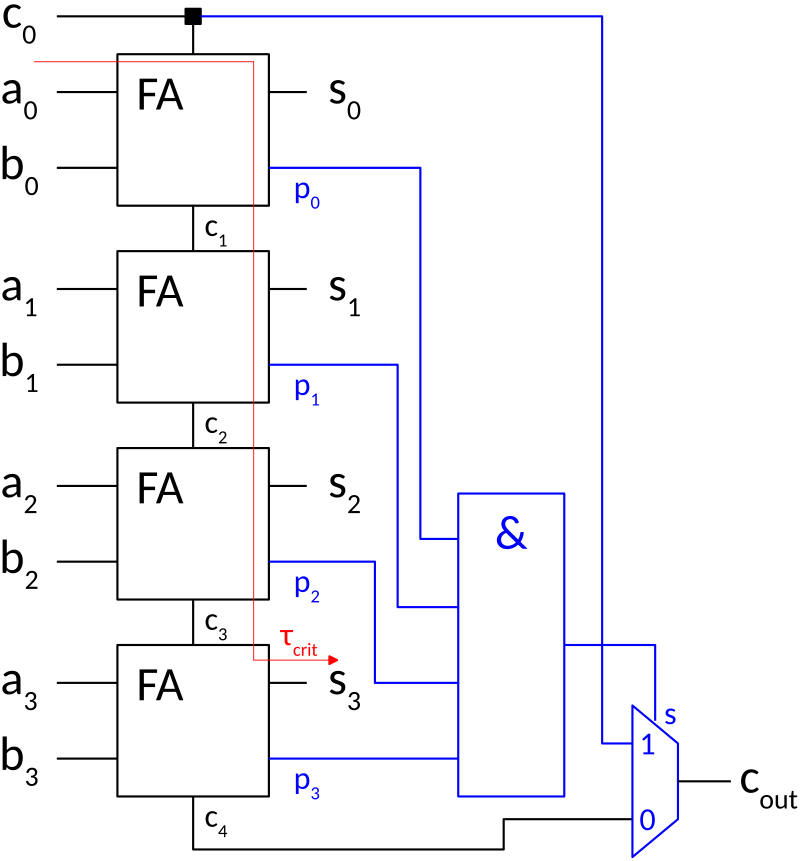
\includegraphics[width = 0.7\textwidth]{CSAdder4Bit.png}
                \caption{Schemat blokowy 4-bit CSA \cite{wikipedia:CSA}.}
                \label{fig:CSA}
            \end{figure}
            Sygnały $S_i$ są poszczególnymi bitami sumy, sygnały pomocnicze 
            $p_i = a_i \oplus b_i$ służą do wyboru przeniesienia wyjściowego. Sygnały przeniesień wewnętrznych są propagowane lub 
            generowane według wzoru:
            \begin{align*}
                c_{i+1} =
                \begin{cases}
                    c_i &\text{jeśli } p_i = 1 \text{ - propagacja}\\
                    a_i &\text{jeśli } p_i = 0 \text{ - generacja}
                \end{cases}
            \end{align*}
            Zastosowanie CSA pozwala obliczyć następny indeks próbki nieco szybciej niż za pomocą standardowych sumatorów. 
            
        \subsubsection{Pamięć próbek}
            Pamięć zrealizowano w postaci dedykowanych programowalnych układów BRAM (\textit{ang.} Block Random-Access Memory). 
            W projekcie wykorzystano pamięć dwu-portową o 10-bitowej magistrali adresowej oraz 64-bitowych komórkach, co odpowiada 
            8192 komórkom po 8 próbkom w każdej. Adresy komórek pamięci odpowiadają indeksom próbek odtwarzanego sygnału. Jeden port pamięci 
            działa w trybie zapisu - służy do ładowania wartości próbek z komputera, 
            a drugi port jest tylko do odczytu - jest adresowany przez akumulator fazy, a odczytane dane są przekazywane do serializerów. 
            Podczas zapisu danych adres kolejnej komórki jest automatycznie inkrementowany na koniec pojedynczej operacji zapisu. Dzięki 
            temu mechanizmowi nie jest potrzebne przesyłanie adresu komórki przez mikroprocesor. 
        \subsubsection{Serializer}
            Do serializacji danych wykorzystano 8 dedykowanych serializerów OSERDESE2 \cite{FPGA_SelectIO}, \cite{AMD_Lib_Guide}, 
            \cite{Zynq_7000_DC_AC} . Pozwalają one osiągnąć znacznie wyższą częstotliwość odtwarzania niż częstotliwość taktowania 
            logiki sterującej. Podczas wystąpienia narastającego zbocza zegara taktującego logikę sterującą - LS\_CLK (Low speed CLK) 
            dane z pamięci są zatrzaskiwane w obwodach wejściowych układów OSERDESE2. Z kolei przy każdym zboczu szybkiego zegara - 
            HS\_CLK (High speed CLK) kolejne bity są przekazywane na wyjście serializerów. Układy OSERDESE2 zostały skonfigurowane do 
            pracy w trybie DDR (\textit{ang.} Double Data Rate) przy szerokości danych wejściowych równej 8 bitów. 
            Pozwala to zmniejszyć częstotliwość zegara HS\_CLK do połowy częstotliwości odtwarzania. W układzie nie jest 
            wykorzystywana praca w trybie trój-stanowym - ogranicza ona szerokość danych do 4 bitów, co wymagałoby stosowania 
            serializerów w trybie master-slave - potrzeba by 2 razy więcej układów OSERDESE2. Przykładowy przebieg serializacji 
            przedstawiono na rysunku \ref{fig:serialization}. Sygnał wyjściowy z serializerów to sample[7:0]. W zaprezentowanym 
            przykładzie układ jest taktowany z dedykowanej pętli fazowej, a wartości próbek są odczytywane z wcześniej zaprogramowanej 
            pamięci BRAM. 
            \begin{figure}[!ht]
                \centering
                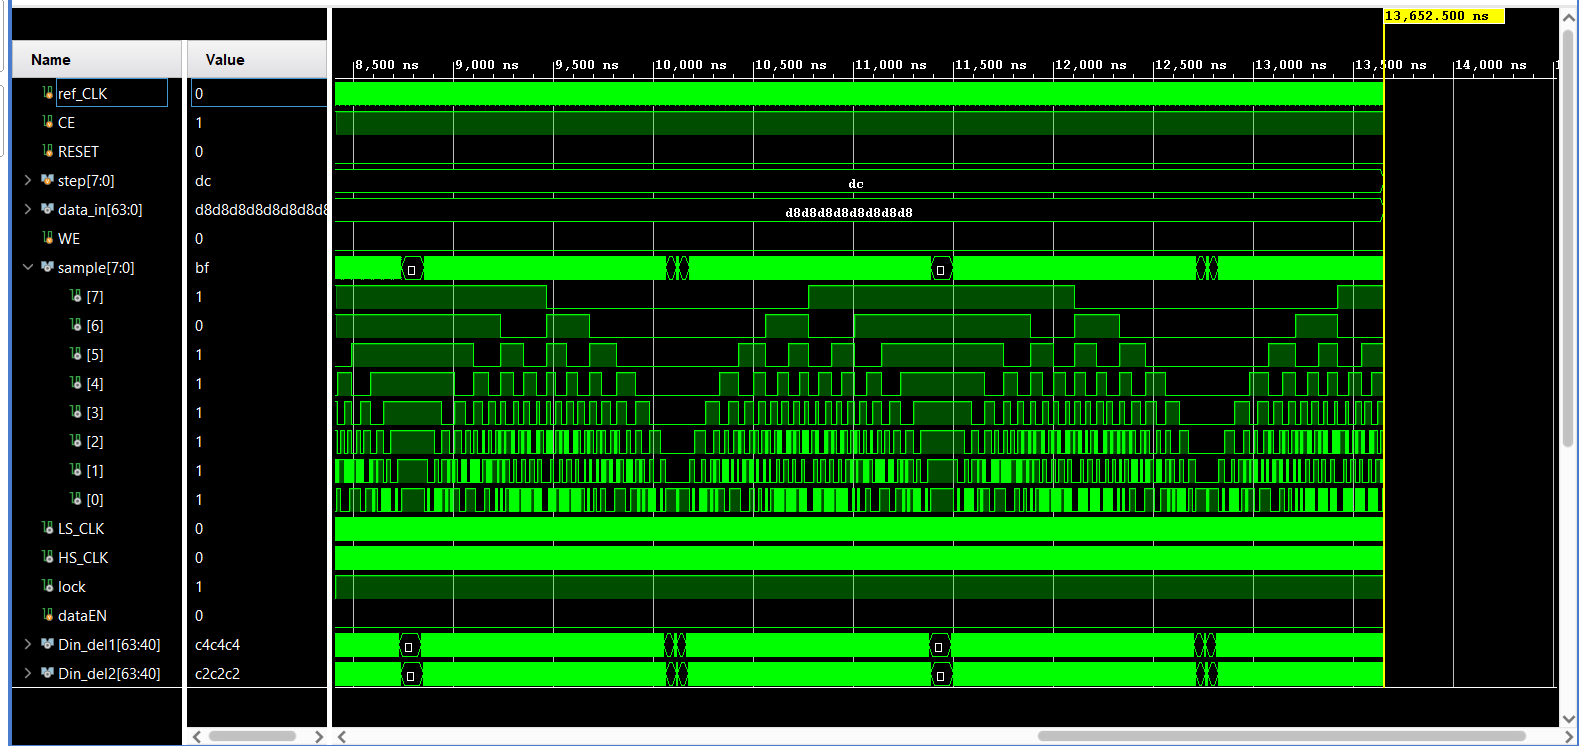
\includegraphics[width = 0.9\textwidth]{sin_serialization.png}
                \caption{Serializacja sygnału sinusoidalnego za pomocą serializera składającego się z 8 układów OSERDESE2 - wynik symulacji czasowej przeprowadzonej po implementacji układu.}
                \label{fig:serialization}
            \end{figure}
        \subsubsection{Generacja zegara}
            Sygnały zegarowe zostały wygenerowane za pomocą dedykowanego układu PLLE2\_BASE. Układ składa się z detektora fazy i 
            częstotliwości - PFD, pompy ładunkowej - CP, filtru dolnoprzepustowego - LF, oraz generatora przestrajanego napięciem - VCO
            oraz głównego dzielnika częstotliwości - M. Ponad to układ posiada aż 6 wyjść zegarowych, każde z nich jest wyposażone 
            w indywidualny dzielnik częstotliwości. Dodatkowo możliwy jest wybór odpowiedniej fazy VCO dla każdego wyjścia niezależnie. 
            Schemat blokowy układu PLLE2\_BASE przedstawiono na rysunku \ref{sch:PLLE2_BASE}.
            \begin{figure}[!ht]
                \centering
                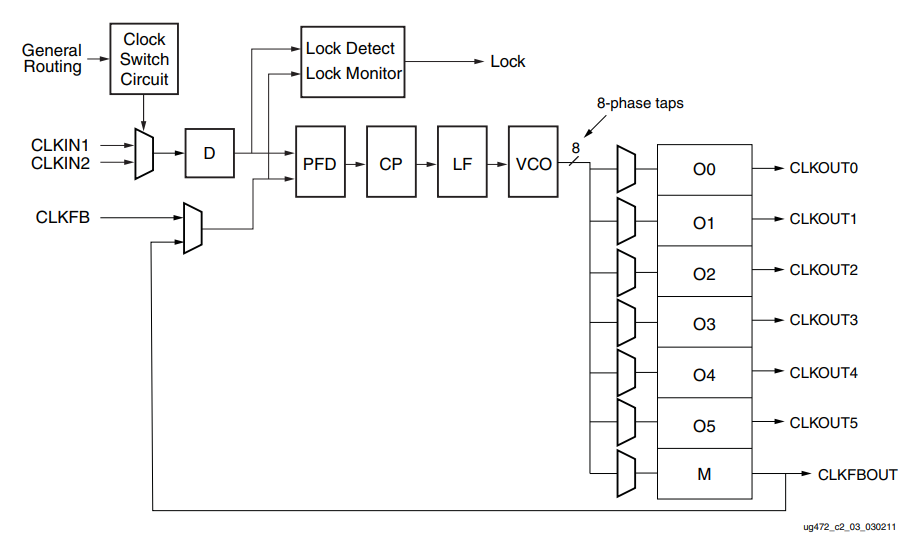
\includegraphics[width = 0.9\textwidth]{PLL2_BASEsch.png}
                \caption{Schemat blokowy układu PLLE2\_BASE \cite{FPGA_Clocking}.}
                \label{sch:PLLE2_BASE}
            \end{figure}
            Wewnętrzny generator przestarajany napięciem może pracować w zakresie $800 \div 2133 \ MHz$. 
            Górna częstotliwość graniczna może się różnić zależnie od możliwości układu FPGA - parametr Grade 
            Speed \cite{Zynq_7000_DC_AC}. Częstotliwość referencyjnego oscylatora kwarcowego umieszczonego na płytce ewaluacyjnej 
            wynosi $f_{REF} = 100\ MHz$ \cite{ZedBoard}. Początkowo zakładano że częstotliwość odtwarzanie sygnału wyniesie $1\ GS/s$, 
            co oznacza, że układy OSERDESE2 pracujący w trybie DDR, należy taktować zegarem $500\ MHz$, z kolei zegar taktujący 
            logikę sterującą miałby częstotliwość 4 razy mniejszą, tj. $125 \ MHz$. Wykorzystując te informacje, skonfigurowano 
            dzielniki częstotliwości pętli fazowej. Dzielnik w sprzężeniu zwrotnym (\textit{ang.} Feedback Divider) ustawiono na $10$, 
            co daje $f_{VCO} = 1000 \ MHz$, a dzielniki wyjściowe ustawiono na $2$ i $8$ odpowiednio dla HS\_CLK i LS\_CLK. 
            Podczas przeprowadzania symulacji wszystko przebiegało prawidłowo, jednak po wygenerowaniu raportu opóźnień, okazało się, 
            że globalne bufory sygnałów zegarowych - BUFG -  nie są w stanie prawidłowo przepropagować sygnału o częstotliwości $500 \ MHz$. 
            Według dokumentacji, ich częstotliwość graniczna wynosi $f_{g_{BUFG}} = 464 \ MHz$ przy speed grade wynoszącym $-1$ \cite{Zynq_7000_DC_AC}. 
            W związku z tym, zmniejszono częstotliwość HS\_CLK do $450 \ MHz$, co daje częstotliwość 
            odtwarzania $900 \ MS/s$. Częstotliwość zegara LS\_CLK również została proporcjonalnie obniżona i wynosi $112.5 \ MHz$. 
            Zmiana częstotliwości wiązała się z modyfikacją konfiguracji dzielników częstotliwości w pętli fazowej - zmniejszono 
            wartość feedback divider'a do $9$, co przekłada się na pracę VCO na częstotliwości $f_{VCO} = 900\ MHz$. Aby uniknąć 
            niezdefiniowanego zachowania układów podczas uruchamiania pętli fazowej, skorzystano z wewnętrznego układu kontrolującego 
            zatrzaśnięcie pętli, a jego sygnał wyjściowy użyto do generowania sygnału CE (\textit{ang.} Clock Enable) w sposób kombinacyjny. 
            Przykładowe przebiegi wyjściowe pętli fazowej zostały przedstawione na rysunku \ref{fig:PLL_clocking}. Istotnym 
            aspektem projektowania ścieżki dystrybucji zegara jest zastosowanie odpowiednich buforów sygnałów zegarowych - dla 
            wszystkich ścieżek powinny zostać użyte takie same bufory w celu uniknięcia wyścigu zboczy. 
            \begin{figure}[!ht]
                \centering
                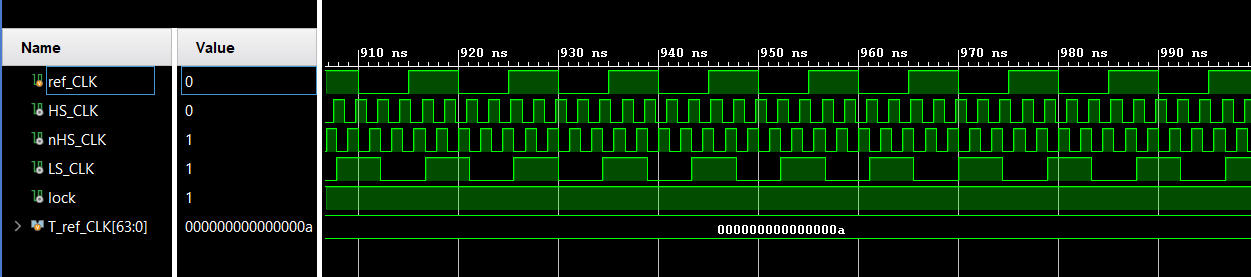
\includegraphics[width = 0.9\textwidth]{PLL_clocking.png}
                \caption{Przebiegi sygnałów zegarowych generowanych przez pętlę fazową - wyniki symulacji czasowej przeprowadzonej po implementacji układu.}
                \label{fig:PLL_clocking}
            \end{figure}

        \subsubsection{Mikroprocesor i protokół UART}
            Mikroprocesor obsługuje kilka poleceń, są to:
            \begin{itemize}
                \item LOAD - przejscie do trybu ładowania danych
                \item STEP - załadowanie kroku fazowego
                \item GENERATE - przejscie do trybu generowania sygnału
                \item BIST - przejscie do trybu testowania
                \item STOP - zatrzymanie pracy układu
                \item RESET - software'owy reset DDS'a
            \end{itemize}
            Wywołanie polecenia powoduje uruchomienie odpowiedniej funkcji oraz przesłanie magistralą AXI odpowiednich 
            sygnałów sterujących to rejestru sterującego. Rozpoznawanie poleceń odbywa się przez ich liczbowe zakodowanie - 
            wystarczy odczytać dwa kolejne bajty. Ładowanie wartości próbek polega na przesyłaniu kolejnych 8-bitowych wartości - próbki 
            mieszczą się w przedziale $0 \div 255$ i przyjmują wartości całkowite. Załadowanie kroku fazowego przebiega analogicznie, 
            z tą różnicą, że jego rozdzielczość jest większa i wynosi $1 \div 4095$. Przesyłane wartości zawsze muszą zawierać 
            odpowiednio 3 lub 4 znaki - odbiór przebiega podobnie jak w przypadku poleceń sterujących. 
        \subsubsection{BIST}
            Układ testujący wykorzystuje 8 generatorów PRBS8 \cite{PRBS8_Thesis} oraz 8 dedykowanych deserializerów ISERDESE2. 
            Generatory PRBS8 pracują równolegle z przesunięciem kroku początkowego o 32. Każdy serializer właściwie działa niezależnie 
            od innych, dlatego nie jest wymagane generowanie sygnału PRBS64, co znacząco wydłużyłoby testowanie - w takim przypadku 
            należałoby ograniczyć liczbę generowanych kodów podczas testu - przy zegarze taktującym $112.5 \ MHz$ sprawdzenie wszystkich 
            możliwych kombinacji zajełoby $\approx 5200$ lat. Znajomość budowy układu, pozwala zredukować liczbę wektorów testowych
            do $2^8$, co przekłada się na czas testu wynoszący zaledwie $\approx 2.3 \ \mu s$. 
            Proces serializacji - deserializacji w obrębie pojedynczego kanału został przedstawiony na rysunku \ref{fig:IOSERDES}. 
            \begin{figure}[!ht]
                \centering
                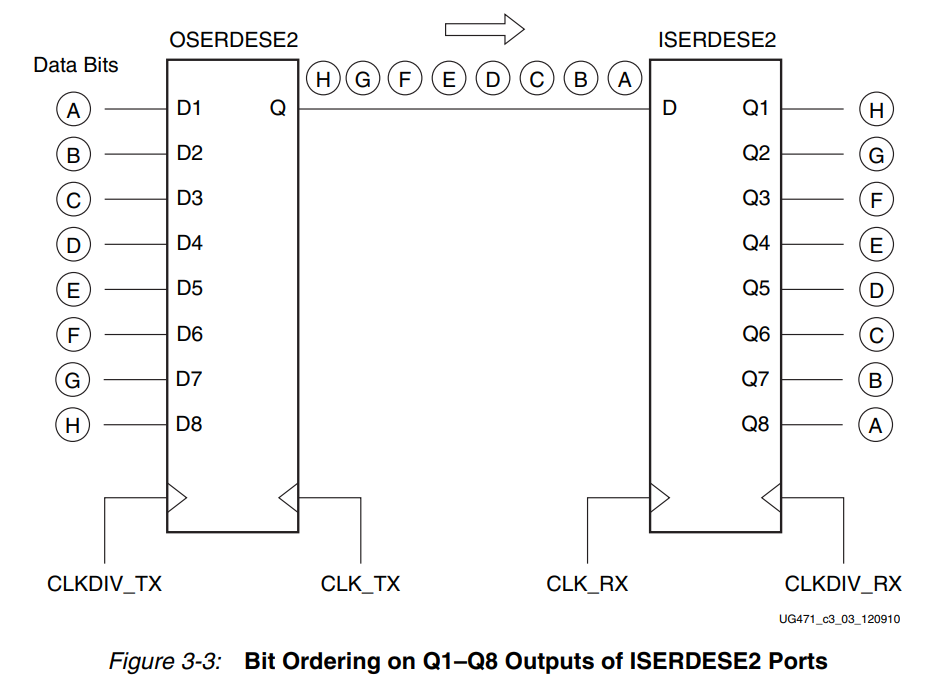
\includegraphics[width = 0.7\textwidth]{BIST_1ch.png}
                \caption{Kolejność przepływu bitów przy serializacji i deserializacji danych za pomocą układów OSERDESE2 i ISERDESE2 \cite{FPGA_SelectIO}.}
                \label{fig:IOSERDES}
            \end{figure}
            Teoretycznie układy OSERDESE2 oraz ISERDESE2 powinny posiadać własne zegary. Podczas projektowania układu okazało się, że 
            nie jest to możliwe - narzędzie do implementacji umieściło układy w obrębie jednego slice'u, co zapewnia niewielkie 
            opóźnienia między serializerem i deserializerem, jednak zabrakło dedykowanych buforów zegara do taktowania układów. 
            W prawdzie platforma Zynq 7000 posiada 32 takie bufory, jednak są one rozdzielone pomiędzy poszczególne slice'y. 
            Rozwiązaniem problemu okazało się zastosowanie tych samych zegarów do taktowania układów - wystarczyło wygenerować 
            zegar HS\_CLK różnicowo. Niestety utrudnieniem okazały się czasy propagacji układów I/OSERDESE2 - w celu prawidłowego 
            porównania  danych serializownych z deserializowanymi należy odczytać 7 bitów z aktualnej sekwencji wyjściowej i 1 najmłodszy 
            bit z poprzedniej oraz sekwencję wzorcową należy opóźnić o 4 takty zegara. Wynik porównania jest realizowany przez 
            komparator kombinacyjny, ale odczyt prawidłowej wartości jest możliwy przy piątym zboczu narastającym LS\_CLK. 
            Przykładowe przebiegi dla symulacji jednego kanału BIST zostały przedstawione na rysunku \ref{fig:BIST_1ch_example}. 
            Dane wejściowe to 8 najstarszych bitów sygnału Din[11:0], sygnał OFB, to sprzęrzenie zwrotne między srerilaizerem, a 
            deserializerem, dane wyjściowe układy ISERDESE2 to sygnał Dout[7:0]. Sygnały Din\_deli stanowią dane wejściowe opóźnione o 
            odpowiednią liczbę taktów zegara. Są one synchroniczne z sygnałem zegarowym LS\_CLK ponieważ są generowane w TestBenchu, 
            a nie wewnątrz testowanego układu. Pozostałe sygnały są synchroniczne z zegarem buforowanym zegarem LS\_CLK. Przykład zrealizowano 
            dla zegara $f_{LS\_CLK} = 125 \ MHz$ ze względu na wymogi środowiska - nie implementowano pętli fazowej, a podstawową jednostką 
            czasu symulacji jest $1 \ ns$ - okres zegara jest całkowitą wielokrotnością podstawowej jednostki czasu. W przypadku 8 kanałów 
            BIST opóźnienie również wynosi 5 taktów LS\_CLK. Poprawność serializacji i deserializacji jest sygnalizowana sygnałem correct. 
            \begin{figure}[!ht]
                \centering
                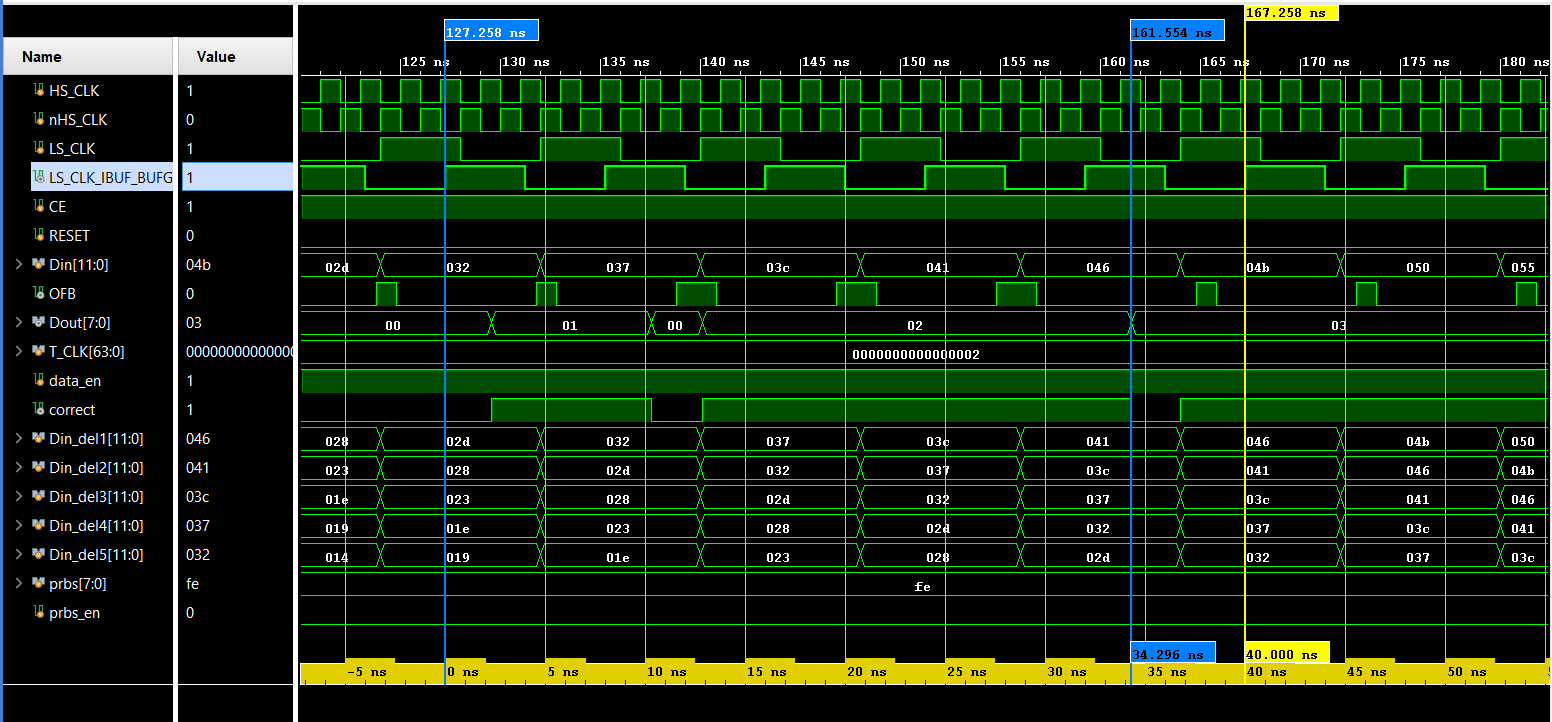
\includegraphics[width = 0.9\textwidth]{BIST_1ch_example.png}
                \caption{Przykładowy przebieg sygnałów dla jednego kanału BIST dla zegara taktującego $125 \ MHz$ - wynik symulacji czasowej przeprowadzonej po implementacji układu.}
                \label{fig:BIST_1ch_example}
            \end{figure}

    \subsection{Przygotowanie próbek}
        Próbki sygnału są przygotowywane za pomocą algorytmu napisanego w języku Python. Skrypt pozwala wygenerować sygnał sinusoidalny, 
        prostokątny, trójkątny oraz piło-kształtny. Użytkownik podaje amplitudę, zdefiniowaną jako procent pełnego zakresu, który 
        wynosi $V_{FS} = 3.3 \ V$, offset zdefiniowany jako procentowa wartość pełnego zakresu oraz liczbę 
        okresów, które mają się zmieścić w pamięci. Wprowadzenie większej amplitudy oraz offsetu jest możliwe, ale będzie się wiązało 
        ze zniekształceniem sygnału w postaci obcięcia wartości wykraczających po za zakres. Użytkownik zostanie o tym poinformowany 
        poprzez wysłanie ostrzeżenia. Algorytm ma zdefiniowaną pojemność pamięci oraz rozdzielczość przetwornika. 
        Wartości próbek są obliczane na podstawie zadanych parametrów - sygnał pseudo-analogowy, a następnie są one normalizowane 
        do pełnego zakresu bitowego i zaokrąglane do wartości całkowitych. Skrypt dodatkowo wyświetla obliczony przebieg w celu 
        weryfikacji i akceptacji, oraz oblicza zalecany zakres kroku fazowego dla proponowanego zestawu próbek. Ma to na 
        celu zredukowanie błędów kwantyzacji oraz redukcję artefaktów występujących w widmie generowanego sygnału - spursów III rzędu. 
        Po akceptacji dane są przesyłane przez port szeregowy do układu FPGA. Na koniec uzytkownik wprowadza krok fazowy. 
        Dodatkowym atutem jest możliwość wyświetlenia dostępnych poleceń wraz z krótkim opisem poprzez wpisanie \textit{help} 
        lub znaku: \textit{?}. 

    
    \subsection{Działanie układu}
        Główny algorytm działania układu został przedstawiony na rysunku \ref{alg:DDSmain}. Sygnały sterujące są przekazywane do 
        rejestrów kontrolnych przez mikroprocesor za pośrednictwem magistrali AXI. W przypadku ładowania próbek do pamięci 
        mikroporcesor ustawia bit WE w rejestrze kontrolnym DDS'a, z kolei układ wewnętrzny generuje impuls pozwalający na 
        zapis otrzymanego pakietu danych trwający dokładnie jeden takt zegara LS\_CLK. Pakiet danych liczy 8 próbek, czyli 64 bity. 
        \begin{figure}[!ht]
            \centering
            \scalebox{0.7}{\begin{subfigure}{\textwidth}
\hspace{0cm}
    \begin{tikzpicture}[node distance = 2cm]

    \node (start) [startstop] {START};
    \node (odczyt) [io, below of = start] {Odczyt rejestrów kontrolnych};
    \node (czyCE) [decision, below of = odczyt, yshift = -1cm] {Czy CE = 1};
    \node (czyLD) [decision, below of = czyCE, yshift = -2.5cm] {Czy załadować dane};
    \node (RD) [io, left of = czyLD, xshift = -4cm] {Odczyt danych};
    \node (LD) [process, below of = RD] {Załadowanie danych};
    \node (Rkrok) [io, below of = czyLD, yshift = -1.5cm] {Odczyt kroku fazowego};
    \node (Lkrok) [process, below of = Rkrok] {Ustawienie kroku fazowego};
    \node (czyGEN) [decision, below of = Rkrok, yshift = -3.5cm] {Czy rozpocząć generację};
    \node (GEN) [process, below of = czyGEN, yshift = -2cm] {Generowanie sygnału};
    \node (stop) [startstop, below of = GEN] {STOP};

    \draw [arrow] (start) -- (odczyt);
    \draw [arrow] (odczyt) -- (czyCE);
    \draw [arrow] (czyCE) --  node[anchor = east]{tak} (czyLD);
    \draw [arrow] (czyCE) -- node[anchor = south]{nie} ++ (4.5, 0) |- (stop);
    \draw [arrow] (czyLD) -- node[anchor = east]{nie} (Rkrok);
    \draw [arrow] (czyLD) -- node[anchor = south]{tak} (RD);
    \draw [arrow] (RD) -- (LD);
    \draw [arrow] (LD) -- ++ (-3.5, 0) |- (odczyt);
    \draw [arrow] (Rkrok) -- (Lkrok);
    \draw [arrow] (Lkrok) -- (czyGEN);
    \draw [arrow] (czyGEN) -- node[anchor = south]{nie} ++ (-9.5, 0) |- (odczyt);
    \draw [arrow] (czyGEN) -- node[anchor = east]{tak} (GEN);
    \draw [arrow] (GEN)  -- ++ (-9.5, 0) |- (odczyt);

    \end{tikzpicture}
\end{subfigure}}
            \caption{Uproszczony algorytm pracy układu.}
            \label{alg:DDSmain}
        \end{figure}

        Wyzwolenie samo-testowania układu powoduje zatrzymania wykonywania głównego algorytmu i przejście do algorytmu BIST. 
        Zostaje on wyzwolony po odczycie danych z rejestrów sterujących, jeśli wystąpił sygnał BIST enable (BIST\_EN). 
        Działanie algorytmu BIST zostało przedstawione na rysunku \ref{alg:BIST}. 
        \begin{figure}[!ht]
            \centering
            \scalebox{0.8}{\begin{subfigure}{\textwidth}
    \hspace{0cm}
    \begin{tikzpicture}[node distance = 2cm]
        \node (start) [startstop] {START};
        \node (odczyt) [io, below of = start] {Odczyt rejestrów kontrolnych};
        \node (czyCE) [decision, below of = odczyt, yshift = -1cm] {Czy CE = 1};
        \node (czyBIST) [decision, below of = czyCE, yshift = -2.5cm] {Czy BIST\_EN = 1};
        \node (czyStop) [decision, left of = czyBIST, xshift = -3cm] {Czy koniec testu};
        \node (SER) [process, below of = czyBIST, yshift = -1.5cm] {Generacja PRBS i serializacja};
        \node (FB) [io, below of = SER] {Odbiór danych serializowanych};
        \node (DES) [process, below of = FB] {Deserializacja danych i porównanie};
        % \node (czyER) [decision, below of = DES] {Czy wystąpił błąd};
        \node (Analyze) [process, below of = DES] {Analiza danych, zmiana sygnałów sterujących};
        \node (summary) [process, below of = Analyze] {Wyślij raport};
        \node (stop) [startstop, below of = summary] {STOP};
        
        \draw [arrow] (start) -- (odczyt);
        \draw [arrow] (odczyt) -- (czyCE);
        \draw [arrow] (czyCE) -- node[anchor = south]{nie} ++ (7, 0) |- (stop);
        \draw [arrow] (czyCE) -- node[anchor = east]{tak} (czyBIST);
        \draw [arrow] (czyBIST) -- node[anchor = south]{nie} ++ (7, 0) |- (stop);
        \draw [arrow] (czyBIST) -- node[anchor = south]{tak} (czyStop);
        \draw [arrow] (czyStop) |- node[anchor = north]{nie} (SER);
        \draw [arrow] (SER) -- (FB);
        \draw [arrow] (FB) -- (DES);
        \draw [arrow] (DES) -- (Analyze);
        \draw [arrow] (Analyze) -- ++ (-9, 0) |- (odczyt);
        \draw [arrow] (czyStop) -- node[anchor = south]{tak} ++ (-3, 0) |- (summary);
        \draw [arrow] (summary) -- (stop);

    \end{tikzpicture}
\end{subfigure}}
            \caption{Algorytm działania BIST.}
            \label{alg:BIST}
        \end{figure}